\chapter{Execution and Results}\label{ch:execandresults}
\epigraph{\textit{ \normalsize“ We dont have better algorithms, we just have more data”}}{\normalsize\textit{Peter Norvig,\\ Director of Research at Google Inc.}}

\section{Training} % (fold)
\label{sec:training}

% section training (end)
Our research consisted of four networks: ACGAN, DCGAN, InfoGAN and WGAN. Each of the networks was trained for 20,000 epochs each. The training period for the individual networks took anywhere between a few hours and a couple of days. For each network, we logged a few key metrics, mainly the Generator Loss (GLoss), Discriminator Loss (DLoss) and the Accuracy (Acc). 
\par\bigskip
Below we show graphically the performance of the (four) classical networks as compared to the CapsNet discriminator augmented networks.

\begin{figure}[H]
    \centering
    \subfloat[Classical ACGAN]{{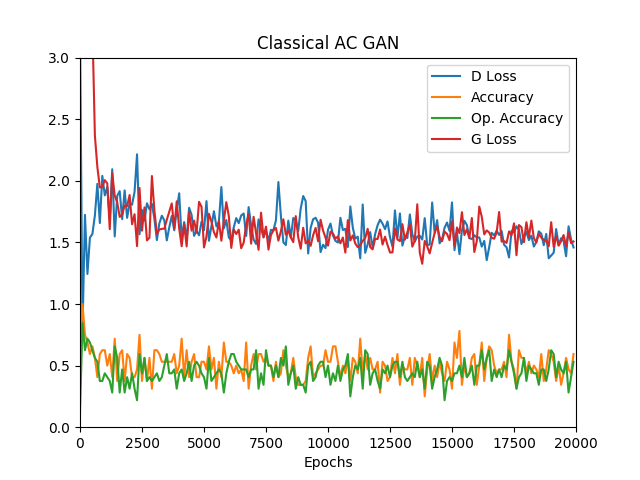
\includegraphics[width=.45\linewidth]{images/plots/classacgan.png} }}%
    \qquad
    \subfloat[CapsNet augmented ACGAN]{{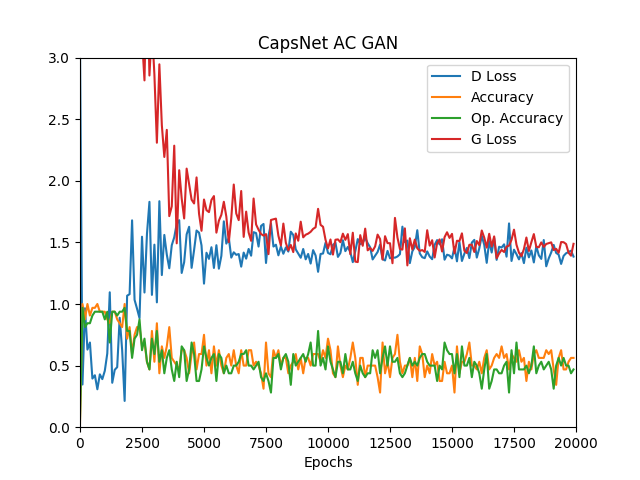
\includegraphics[width=.45\linewidth]{images/plots/capsacgan.png} }}%
    \caption{ACGAN metrics}%
    \label{fig:acgan_metric}%
\end{figure}

\begin{figure}[H]
    \centering
    \subfloat[Classical DCGAN]{{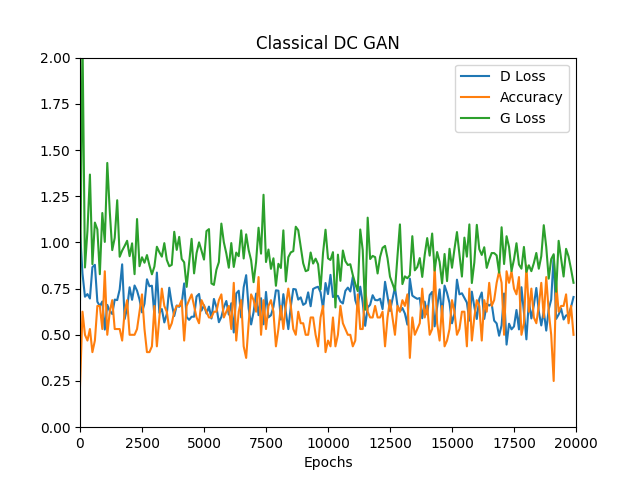
\includegraphics[width=.45\linewidth]{images/plots/classdcgan.png} }}%
    \qquad
    \subfloat[CapsNet augmented DCGAN]{{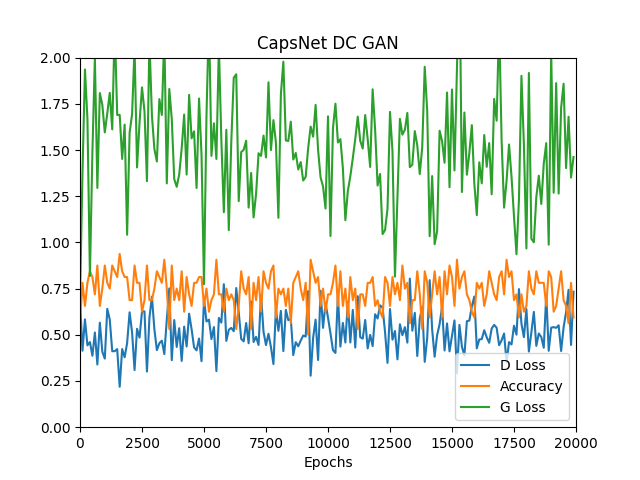
\includegraphics[width=.45\linewidth]{images/plots/capsdcgan.png} }}%
    \caption{DCGAN metrics}%
    \label{fig:dcgan_metric}%
\end{figure}

\begin{figure}[H]
    \centering
    \subfloat[Classical InfoGAN]{{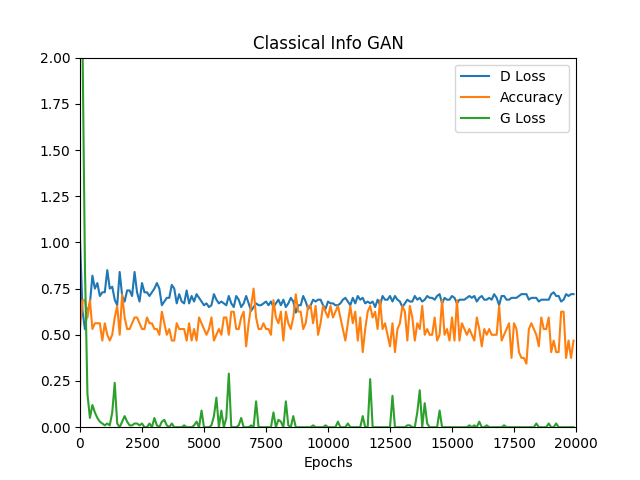
\includegraphics[width=.45\linewidth]{images/plots/classinfogan.png} }}%
    \qquad
    \subfloat[CapsNet augmented InfoGAN]{{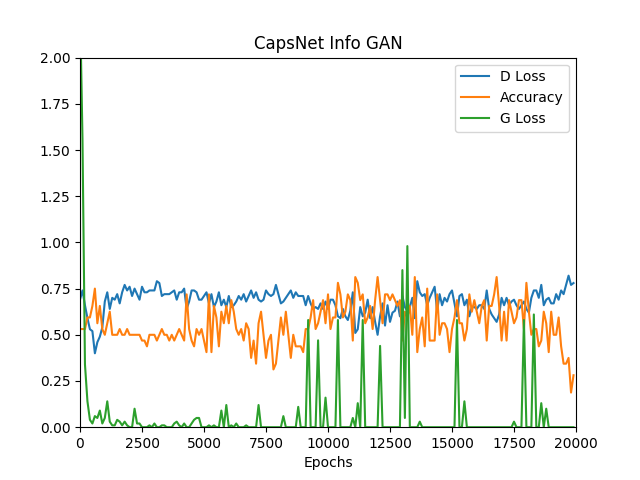
\includegraphics[width=.45\linewidth]{images/plots/capsinfogan.png} }}%
    \caption{InfoGAN metrics}%
    \label{fig:infogan_metric}%
\end{figure}

\begin{figure}[H]
    \centering
    \subfloat[Classical WGAN]{{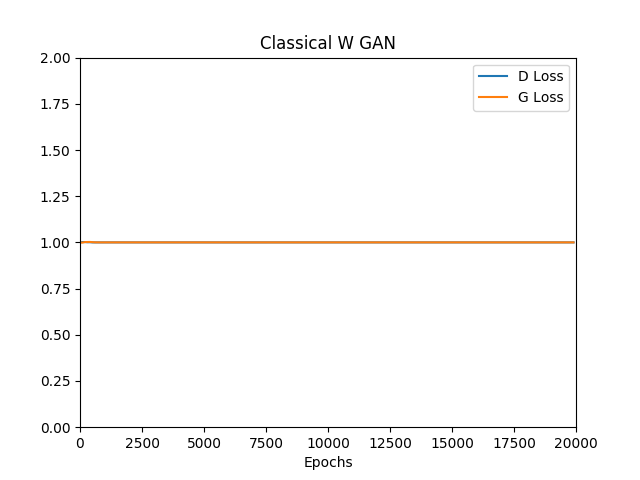
\includegraphics[width=.45\linewidth]{images/plots/classwgan.png} }}%
    \qquad
    \subfloat[CapsNet augmented WGAN]{{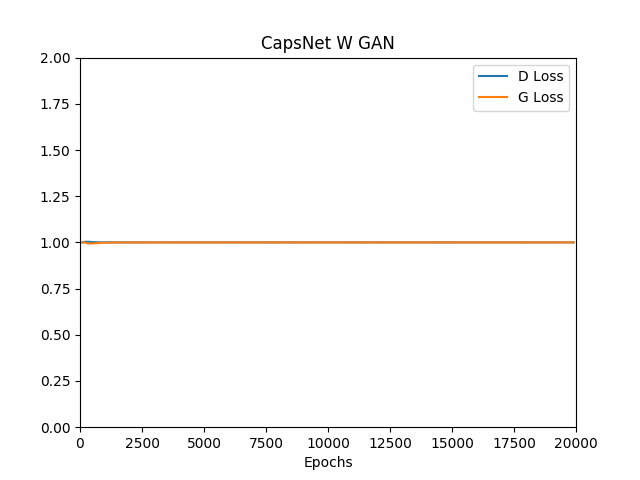
\includegraphics[width=.45\linewidth]{images/plots/capswgan.png} }}%
    \caption{WGAN metrics}%
    \label{fig:wgan_metric}%
\end{figure}

The metrics of WGAN are at a smaller scale, so below is a comparison at the lower scale.

\begin{figure}[H]
    \centering
    \subfloat[Classical WGAN]{{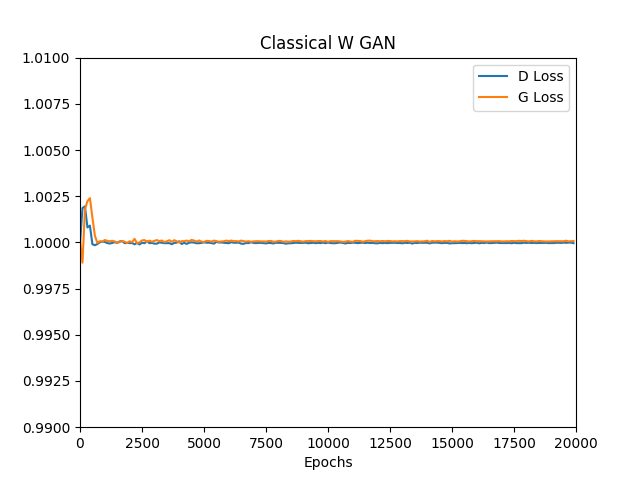
\includegraphics[width=.45\linewidth]{images/plots/classwgan-zoomed.png} }}%
    \qquad
    \subfloat[CapsNet augmented WGAN]{{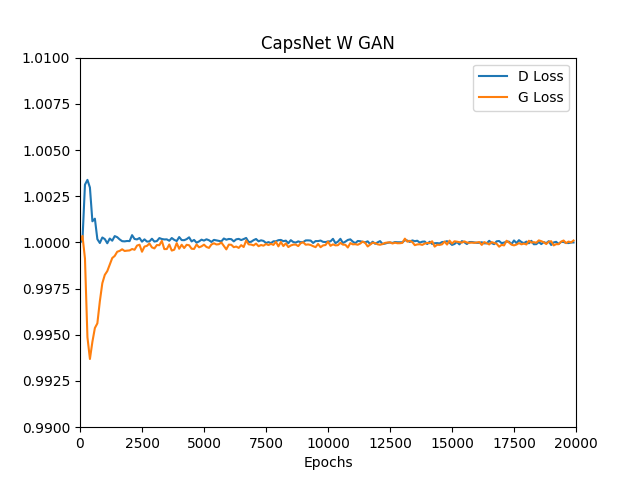
\includegraphics[width=.45\linewidth]{images/plots/capswgan-zoomed.png} }}%
    \caption{WGAN metrics - zoomed}%
    \label{fig:wgan_metric_zoomed}%
\end{figure}
\par\bigskip

A preliminarily analysis of the data shows us that our CapsNet augmented networks, hence-forth referred to as the network name prefixed with "Caps", perform comparably with the classical architectures. 
\par\bigskip

Under ACGAN we see that CapsACGAN starts off with very high variance in GLoss and DLoss. Over the course of 20,000 epochs, the variance gradually reduces to match the Classical ACGAN metrics at the end. Accuracy of CapsACGAN, on the other hand, quickly stabilizes to meet classical ACGAN metrics. As a side note, ACGAN was the fastest trained network, taking roughly three hours to complete 20,000 epochs.
\par\bigskip

DCGAN and InfoGAN are interesting in the sense that they show a remarkable shift in the GLoss metric. Even though it seems as if augmenting DCGAN with CapsNet discriminator leads to increase in GLoss, a closer look reveals that increased variation leads to faster learning of the generator network. Accuracy and DLoss follow their classical counterpart closely.
\par\bigskip

WGAN happens to be the best and state-of-the-art. Consequently, the variance in the metrics were at a much smaller scale, that is, the network is designed to be more stabilized and balanced but this also leads to slower learning, we can see that adding CapsNet discriminator speeds this up by adding slightly more variance while the network is still balanced. We had to zoom-in to notice the difference between the metrics. We see that an initial burst of high variance quickly stabilizes to trace a path closely matching the classical architecture.
\par\bigskip
\newpage

\section{Generation} % (fold)
\label{sec:generation}
At the end of every epoch we saved the outputs of the generator. Here we show the outputs of generator of four networks after 20,000 epochs for comparison.
\begin{figure}[H]
    \centering
    \subfloat[Classical ACGAN]{{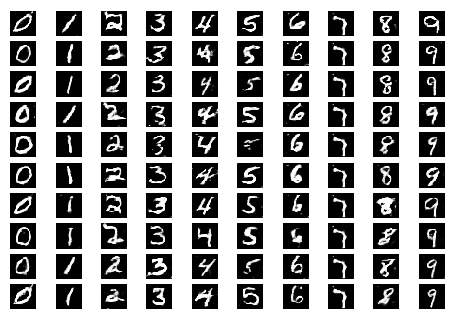
\includegraphics[width=.49\linewidth]{images/generation_outputs/acgan.png} }}%
    \subfloat[CapsNet augmented ACGAN]{{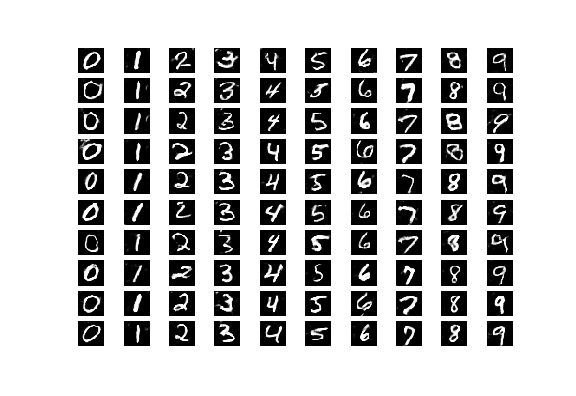
\includegraphics[width=.49\linewidth]{images/generation_outputs/acgan_caps.png} }}%
    \caption{ACGAN outputs}%
    \label{fig:acgan_gen}%
\end{figure}
As expected from the metrics the ACGAN and CapsACGAN produce very similar outputs.
\begin{figure}[H]
    \centering
    \subfloat[Classical DCGAN]{{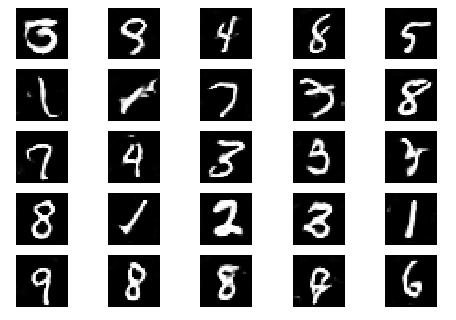
\includegraphics[width=.45\linewidth]{images/generation_outputs/dcgan.png} }}%
    \qquad
    \subfloat[CapsNet augmented DCGAN]{{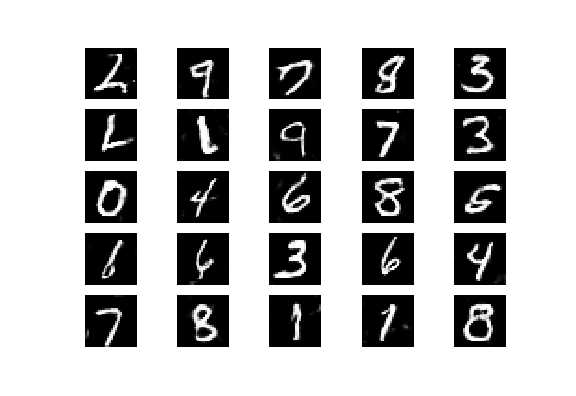
\includegraphics[width=.45\linewidth]{images/generation_outputs/dcgan_caps.png} }}%
    \caption{DCGAN outputs}%
    \label{fig:dcgan_gen}%
\end{figure}
The outputs of DCGAN and CapsDCGAN are almost indistinguishable but a closer look reveals that CapsDCGAN produces more clear outputs and more percentage of CapsDCGAN outputs look real.

\begin{figure}[H]
    \centering
    \subfloat[Classical InfoGAN]{{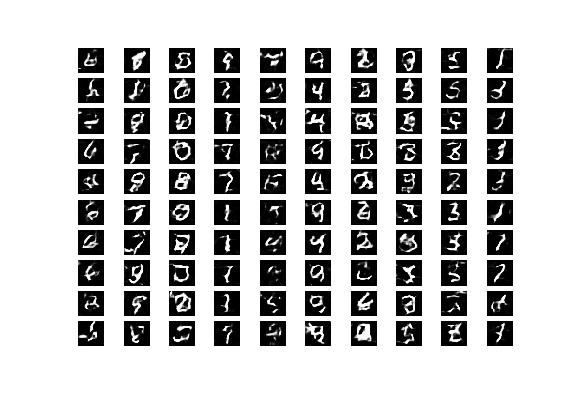
\includegraphics[width=.49\linewidth]{images/generation_outputs/infogan.png} }}%
    \subfloat[CapsNet augmented InfoGAN]{{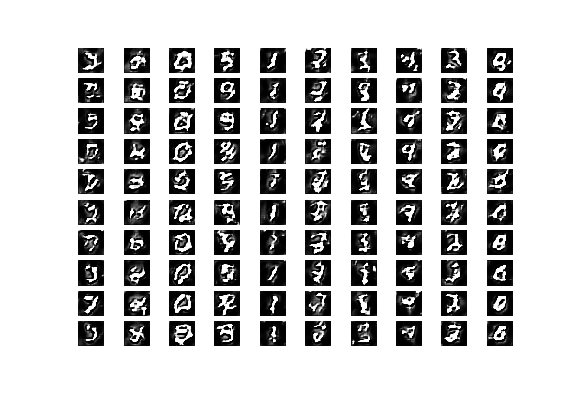
\includegraphics[width=.49\linewidth]{images/generation_outputs/infogan_caps.png} }}%
    \caption{InfoGAN outputs}%
    \label{fig:infogan_gen}%
\end{figure}
Even though the CapsInfoGAN output looks structurally better and has learned faster but it is more noisier than that of the InfoGAN.
\begin{figure}[H]
    \centering
    \subfloat[Classical WGAN]{{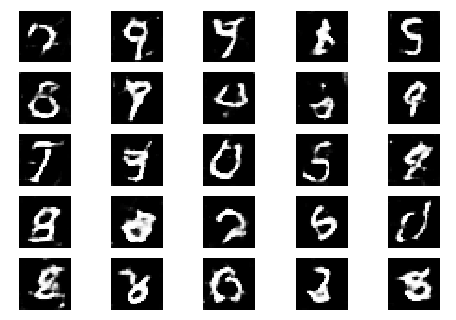
\includegraphics[width=.42\linewidth]{images/generation_outputs/wgan.png} }}%
    \qquad
    \subfloat[CapsNet augmented WGAN]{{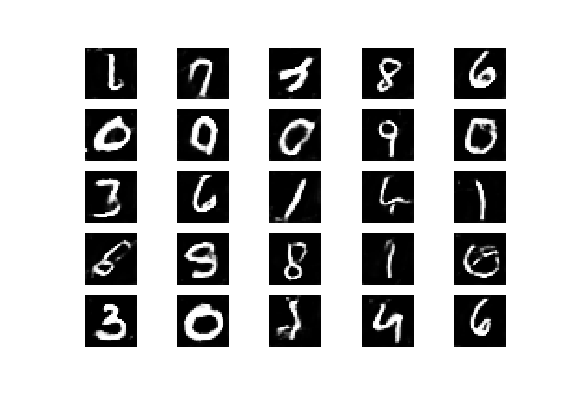
\includegraphics[width=.42\linewidth]{images/generation_outputs/wgan_caps.png} }}%
    \caption{WGAN outputs}%
    \label{fig:wgan_gen}%
\end{figure}
Finally in the WGAN outputs we can clearly see that CapsWGAN produces clear and better outputs, hence has learned more quickly than the WGAN. 

% section generation (end)
\newpage

\section{Demonstration} % (fold)
\label{sec:res_demonstration}

Initially, for demonstration of semantic in-painting, we used the MNIST model of CapsDCGAN that we used in the previous sections. We had promising results as seen in the figure \ref{fig:mnist_examples}.

\begin{figure}[H]
    \centering
    \subfloat{{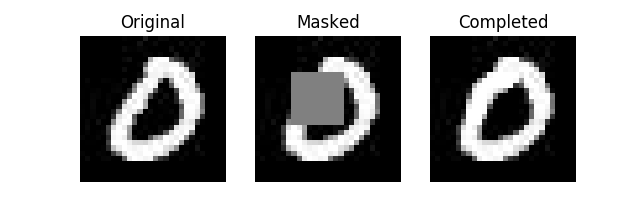
\includegraphics[width=.49\linewidth]{images/completion_outputs/0_1.png} }}%
    \subfloat{{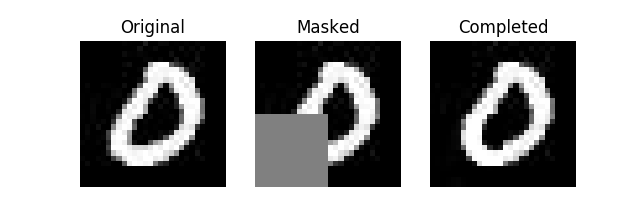
\includegraphics[width=.49\linewidth]{images/completion_outputs/0_2.png} }}%
    \\
    \centering
    \subfloat{{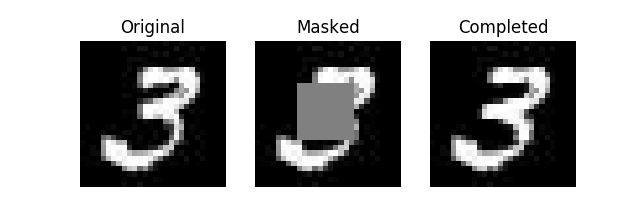
\includegraphics[width=.49\linewidth]{images/completion_outputs/3_1.png} }}%
    \subfloat{{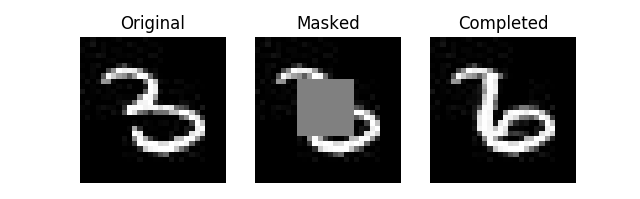
\includegraphics[width=.49\linewidth]{images/completion_outputs/3_2.png} }}%
    \\
    \centering
    \subfloat{{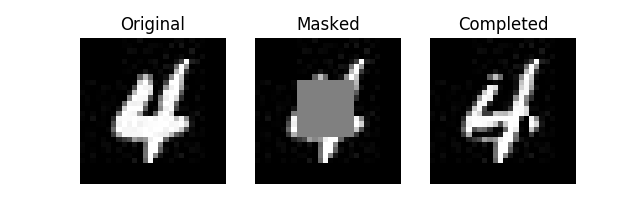
\includegraphics[width=.49\linewidth]{images/completion_outputs/4.png} }}%
    \subfloat{{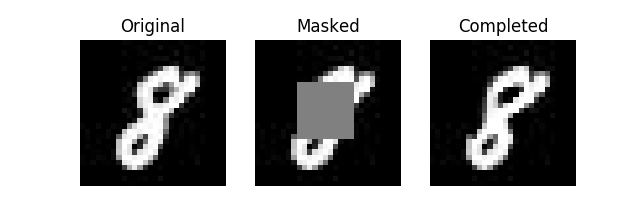
\includegraphics[width=.49\linewidth]{images/completion_outputs/8_1.png} }}%
    \\
    \centering
    \subfloat{{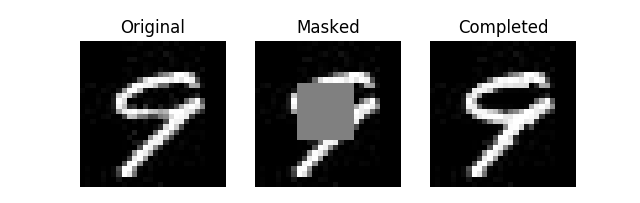
\includegraphics[width=.49\linewidth]{images/completion_outputs/9_1.png} }}%
    \caption{MNIST examples}%
    \label{fig:mnist_examples}%
\end{figure}

\newpage
For the completion of faces however the process was more complex. We initially trained CapsDCGAN on LFW dataset \cite{lfw} for 50 epochs. Since LFW contains only 13,233 images, the model suffered from low generalization. So we decided to use the larger CelebA dataset \cite{celeba} for training. CelebA consists of 202,599 images of 10,177 celebrities. We trained CapsDCGAN on CelebA for only 9 epochs and still obtained realistic images. The following are the completion outputs from CelebA model in figure \ref{fig:face_examples}.
\begin{figure}[H]
    \centering
    \subfloat{{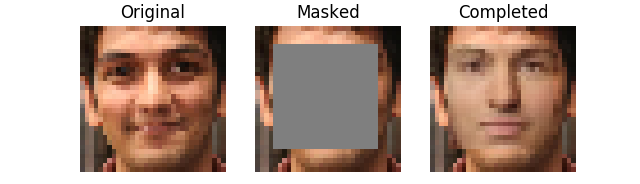
\includegraphics[width=.49\linewidth]{images/completion_outputs/Figure_10.png} }}%
    \subfloat{{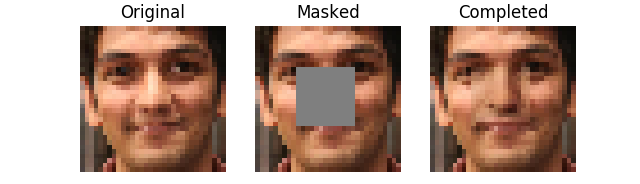
\includegraphics[width=.49\linewidth]{images/completion_outputs/Figure_11.png} }}%
    \\
    \centering
    \subfloat{{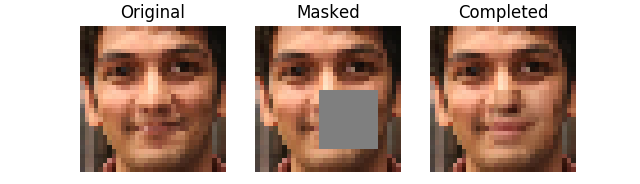
\includegraphics[width=.49\linewidth]{images/completion_outputs/Figure_12.png} }}%
    \subfloat{{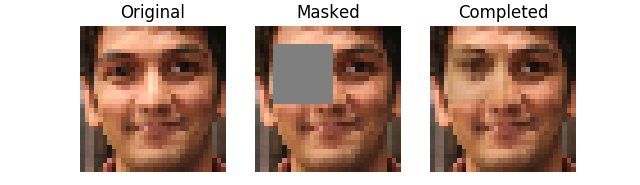
\includegraphics[width=.49\linewidth]{images/completion_outputs/Figure_13.png} }}%
    \\
    \centering
    \subfloat{{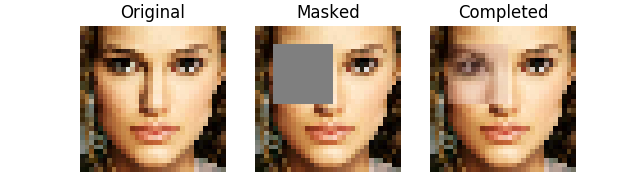
\includegraphics[width=.49\linewidth]{images/completion_outputs/Figure_14.png} }}%
    \subfloat{{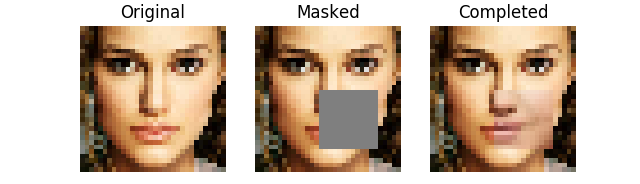
\includegraphics[width=.49\linewidth]{images/completion_outputs/Figure_15.png} }}%
    \\
    \centering
    \subfloat{{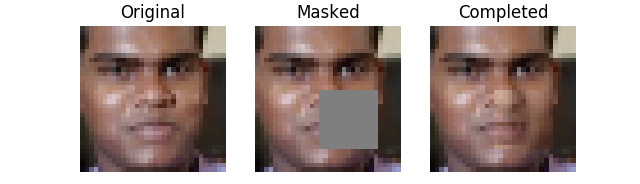
\includegraphics[width=.49\linewidth]{images/completion_outputs/Figure_16.png} }}%
    \subfloat{{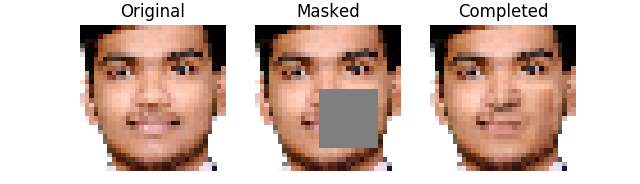
\includegraphics[width=.49\linewidth]{images/completion_outputs/Figure_17.png} }}%
    \\
    \centering
    \subfloat{{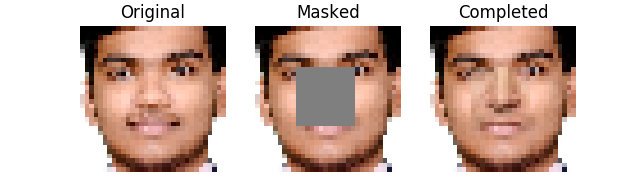
\includegraphics[width=.49\linewidth]{images/completion_outputs/Figure_18.png} }}%
    \subfloat{{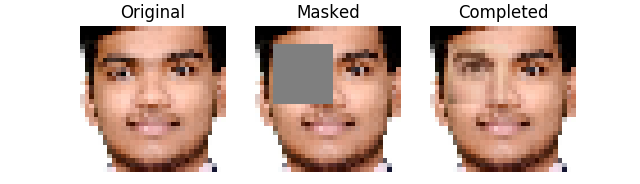
\includegraphics[width=.49\linewidth]{images/completion_outputs/Figure_19.png} }}%
    \\
    \centering
    \subfloat{{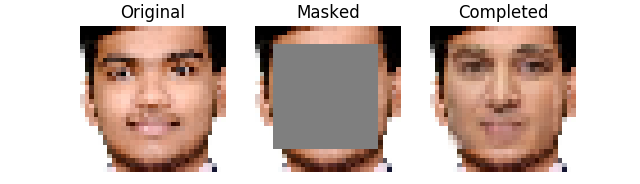
\includegraphics[width=.49\linewidth]{images/completion_outputs/Figure_20.png} }}%

    \caption{Face examples}%
    \label{fig:face_examples}%
\end{figure}

\newpage
To facilitate demonstration and visual appeal we ported our completion code into a webapp using flask and socketio. The webapp provides a way to select images, draw a mask on them, and execute completion code. When performing the projected gradient descent, the webapp displays the dynamic state of the completed image, the number of iterations, and the graph of the loss function respect to the iteration, these values are dynamically updated using socketio, which is a Web-socket library. Web-socket provides a bidirectional communication channel between the client and the server. \par\bigskip
\begin{figure}[H]
\centering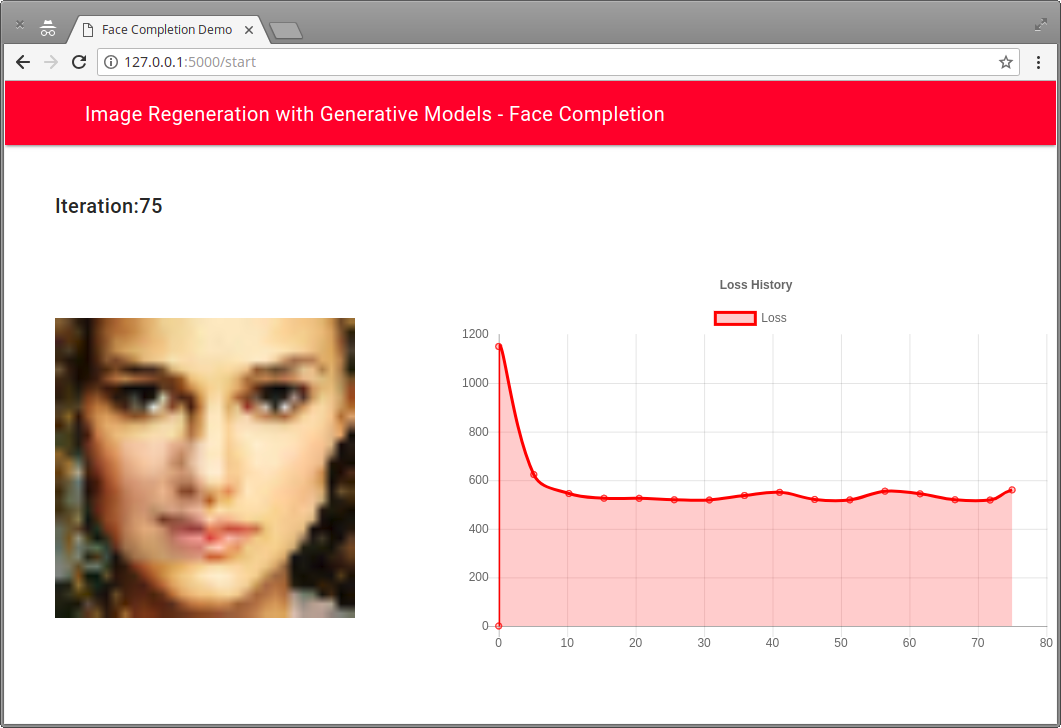
\includegraphics[width=1\textwidth]{images/DemoFrontend.png}
\caption{Demonstration WebApp Interface}
\label{fig:demo}
\end{figure}